%%% File encoding is UTF8

\chapter{Desarrollo}

Este capítulo es de prueba de las capacidades que tiene \LaTeX y que se ofrecen en este proyecto.

\section{Tablas}

Como se puede apreciar en la \tab{tab:ex1}.

\insertTableFile{Ejemplo de una tabla leída desde CSVexample.csv.}{\fuentePropia}{04_Tables/CSVexample.csv}{\label{tab:ex1}}

\begin{table}[htb]
	\centering
	\captiontable{A small table created with the \texttt{booktabs} package (example taken from the package documentation).}{\fuentePropia}
	\begin{tabular}{@{}llr@{}} \toprule
		\multicolumn{2}{c}{Item} \\ \cmidrule(r){1-2}
		Animal & Description & Price (\$)\\ \midrule
		Gnat & per gram & 13.65 \\
		& each & 0.01 \\
		Gnu & stuffed & 92.50 \\
		Emu & stuffed & 33.33 \\
		Armadillo & frozen & 8.99 \\ \bottomrule
	\end{tabular}
\end{table}

%\begin{figure}[htb]
%	\centering
	%Picture
%	\input{03_GraphicFiles/02_Desarrollo/tikz-example}
%	\captionsource{Figura de ejemplo realizada en Tikz}{\fuentePropia}
%	\label{fig:tikz-example}
%\end{figure}

\sisetup{table-format=2.2} 
\begin{table}
	\centering
	\captiontable{Precision y Recall.}{\fuentePropia}
	\begin{tabular}{|c|l|S|S|S|S|}           \hline 
		\multirow{2}{*}{\# of class} &\multirow{2}{*}{type}    & \multicolumn{2}{c|}{Trained Data}    &\multicolumn{2}{c|}{New Data}                    \\   \cline{3-6}
		&  &{Prec.} & {Rec.} & {Prec.}  & {Rec.}              \\   \hline 
		\multirow{5}{*}{5} & car& 81.8 &73.1 & 73.8   & 46.3   \\   \cline{2-6}  
		& plane & 88.3 & 80.7 & 81.1   & 72.5                 \\   \cline{2-6} 
		& camera & 98.1 & 96.4 & 95.2   &  87                 \\   \cline{2-6} 
		& cup & 42.2 & 37.5 & 31   &   22.6                   \\   \cline{2-6} 
		& landscape & 71.7 & 44.9 & 67.9   & 54.3             \\   \hline 
		\multicolumn{2}{|c|}{Average}   & 76.42 & 66.52 &69.8 & 56.54 \\ \hline 
	\end{tabular}
\end{table}

\section{Figuras}

\begin{figure}
	\centering
	\subcaptionbox{left\label{sub-left}}{%
		\includegraphics[height=175bp,width=.45\textwidth]{example-image}%
	}\hfil
	\subcaptionbox{right\label{sub-right}}{%
		\includegraphics[height=175bp,width=.45\textwidth]{example-image}%
	}
	
	\captionsource{Dos figuras (a) y (b).}{\fuentePropia}
\end{figure}

\begin{figure}[htb]
	\centering
	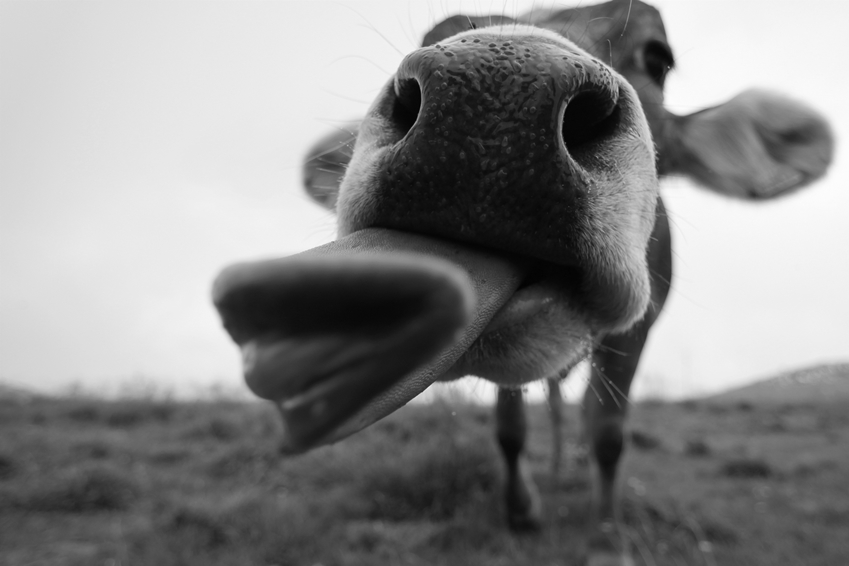
\includegraphics[width=0.9\textwidth]{03_GraphicFiles/CowLickingNose.jpg}
	\captionsource{A cow licking its nose. Usage with permission of the photographer \textsc{Nicole Barth}}{Obtenido de \url{www.flickr.com/photos/46311827@N07/14885545396}, (2017)}
	\label{fig:CowLickingNose}
\end{figure}


%\plotFile{x}{y}{07_DataForPlot/ej-data-plot.txt}
\begin{figure}[htb]
	\centering
	\begin{tikzpicture}
	\begin{axis}[unit vector ratio=1 1 % same size for both unit axis vectors
				, ylabel={Correct Codes}
				, ylabel style= {yshift=-4mm,}
				, xlabel={Keyword Frequency (Code)}
				, width = 0.9\textwidth
				, height= 80mm
				, cycle list name=Dark2
				, grid=major
				, legend pos=outer north east
				, legend style= {cells={anchor=west}, outer ysep=0pt}
				, xmin=0
				, xmax=11.5
				, ymin=0
				, every axis plot post/.style={very thick}
				, grid style=dashed
				, title style={font=\bfseries,align=center,text width=0.7\textwidth}
				, title = {Diagrama de ejemplo}
				]

\addplot+[smooth, mark=*] coordinates {(1,5)(2,5)(3,4)(4,5)(5,5)(6,5)(7,5)(8,5)(9,5)(10,5)};
\addplot+[smooth, dashed, mark=square*, mark options={solid}] coordinates {(1,9)(2,6)(3,6)(4,5)(5,4)(6,5)(7,6)(8,5)(9,5)(10,5)};
\addplot+[smooth, dotted, mark=triangle*, mark options={solid}] coordinates {(1,6)(2,7)(3,7)(4,6)(5,7)(6,9)(7,10)(8,10)(9,9)(10,9)};
\addplot+[smooth, densely dashed, mark= diamond*, mark options={solid}] coordinates {(1,7)(2,6)(3,5)(4,5)(5,7)(6,4)(7,4)(8,4)(9,4)(10,5)};

\legend{WordCount,KeywordRelevance,KeywordCount,DISCOKeywords}
\end{axis}
\end{tikzpicture}
\captionsource{Plot realizado con Tikz usando como colores Dark2}{\fuentePropia}
\label{fig:plot-example}
\end{figure}

\section{Ecuaciones}
\label{sec:equations}
This is how a equation looks like in this document:

\begin{equation}
\cos (2\theta) = \cos^2 \theta - \sin^2 \theta
\end{equation}

\begin{equation}
	F1 = \frac{2 \cdot Precision\cdot Recall}{Precision+ Recall}
\end{equation}

\begin{equation}
	Precision = \frac{TP}{TP+ FP}
\end{equation}

\begin{equation}
	Precision = \frac{\big[\big\{documentos \ relevantes\big\} \cap \big\{documentos \ recuperados\big\}\big]}{\big\{documentos \ recuperados\big\}}
\end{equation}

\begin{equation}
	Recall = \frac{TP}{TP+ FN}
\end{equation}

\begin{equation}
	Recall = \frac{\big[\big\{documentos \ relevantes\big\} \cap \big\{documentos \ recuperados\big\}\big]}{\big\{documentos \ relevantes\big\}}
\end{equation}

\section{Algoritmos}

\begin{algorithm}[hbt]
	\caption{Escribiendo algoritmos usando \LaTeX2e}
	\SetAlgoLined
	\KwIn{Esto es la entrada del algoritmo}
	\KwOut{Esto es la salida del algoritmo}
	%\KwData{Esto son los datos con que trabaja el algoritmo}
	%\KwResult{Esto es el resultado del algoritmo}
\Begin{
	$V \longleftarrow U$\;
	$S \longleftarrow \emptyset$\;

	\While{not at end of this document}{
		read current\;
		\eIf{understand}{
			go to next section\;
			current section becomes this one\;
		}{
			go back to the beginning of current section\;
		}
	}
}	
\end{algorithm}

\section{Citas}

Para citar ocupar la siguiente forma: 

\begin{itemize}
	\item \cite{Codishetal2000}.
	\item Ej: \textcite{Codishetal2000} menciona que.
\end{itemize}

La bibliografía saldrá dependiendo del tipo de documento citado.

\begin{description}
	\item[Articulo de revista] Iniciales y Apellido del autor, "Título del artículo entre comillas," \textit{Título abreviado de la revista en cursiva}, volumen (abreviado vol.), número abreviado no.), páginas (abreviado pp.), Mes, Año.
	\item[Monografía] Iniciales y Apellido, \textit{Título del libro en cursiva}, Edición. Lugar de publicación: Editorial, Año de publicación.
	\item[Manual técnico] \textit{Título en cursiva del manual}, Edición. Nombre de la empresa, Sede de la empresa, Año de publicación.
	\item[Informes técnicos] Iniciales y Apellido del Autor, "Título del informe entre comillas," Nombre de la empresa, Sede de la empresa, Tipo de informe abreviado, Número de informe, Fecha de publicación.
	\item[Capítulo de un libro] Iniciales y Apellido del Autor, "Título del capítulo entre comillas,". en \textit{Título del libro en cursiva}, Iniciales y Apellido del Editor, Compilador. etc. Editorial: Lugar de publicación, Año de publicación, Páginas (abreviadas pp.)
	\item[Artículo de revista] Iniciales y Apellido del autor, "Título del artículo entre comillas", \textit{Título abreviado de la revista en cursiva}, volumen (abreviado vol.), número abreviado no.), páginas (abreviado pp.), Mes, Año
	\item[Recurso de Internet] Igual que los documentos impresos, añadiéndoles la indicación [online] y el DOI (Digital Object Identifier), que generalmente se corresponde con la URL.
	\item[Documentos ineditos] Iniciales y Apellido del autor, "Título entre comillas," Clase de documento (tesis doctoral, trabajo fin de carrera...), Departamento, Institución académica, Ciudad, Año
\end{description}




\section{Gantt}


\begin{figure}[H]
\centering
\label{tabla:estado-avance}
\scalebox{0.9} {
\begin{ganttchart}[
	today=4
	]{1}{19}
	
	\gantttitle{Proyecto tesis}{19}\\
	\gantttitle[]{2017}{19} \\               
	
	\gantttitle{Mar}{4}                     
	\gantttitle{Abr}{4}
	\gantttitle{May}{4}
	\gantttitle{Jun}{4}
	\gantttitle{Jul}{3} \\ % Fin: Entrega 12 julio 2017
	
	\ganttgroup[inline=false]{Diseño de la arquitectura}{1}{8} \\ 
	\ganttbar[progress=70,inline=false]{Fase de pruebas}{1}{8} \\
	
	\ganttgroup[inline=false]{Diseño de algoritmo de planificación}{1}{19} \\ 
	\ganttbar[progress=50,inline=false]{Evaluación de los algoritmos}{1}{16} \\
	\ganttbar[progress=40,inline=false]{Obtención de resultados}{1}{16} \\
	\ganttbar[progress=40,inline=false]{Generación de gráficos}{1}{16} \\
	\ganttbar[progress=30,inline=false]{Comparación de resultados}{12}{19} \\
	\ganttbar[progress=20,inline=false]{Obtener conclusiones del trabajo}{16}{19} \\
	
	\ganttgroup[progress=70, inline=false]{Redacción del documento}{1}{19} \\ 
\end{ganttchart}	
}
\captionsource{Carta Gantt propuesta.}{\fuentePropia}
\end{figure}



%\section{Destacar cambios}
%Esto es un \correcion{cambio realizado y marcado}.